% !TeX encoding = UTF-8
% !TeX program = pdflatex

\documentclass[12pt]{article}
\usepackage{hyperref}
\usepackage{graphicx}
\usepackage{graphics}
\usepackage{listings}
\usepackage{amsmath}
\usepackage{verbatim}
\usepackage{tikz}
\usepackage{caption}
\usepackage{pgfplots}
\usepackage{dirtree}

\captionsetup[figure]{font=scriptsize,labelfont=scriptsize}

\pgfplotsset{compat=1.14}

\hypersetup{
    colorlinks,
    citecolor=black,
    filecolor=black,
    linkcolor=black,
    urlcolor=black
}

\renewcommand{\baselinestretch}{1.15}

\title{{\bf Weather Classification} \\ \bigskip \large HW2 - Machine Learning \\ \large "Sapienza" University of Rome}
\author{Valerio Coretti 1635747}

\begin{document}
\maketitle

\section{Introduction}
Neural networks are the basis of deep learning, and while they may look like black boxes, they are basically trying to get the same thing as any other model to make good predictions. In this homework we want to solve the problem of the {weather calssification}, in particular we have to recognize the weather from an image.

To do this we used Neural Networks approach. We had a dataset with 4000 images. Each image belong to a class. Therefore the problem is a Multiclass Classification problem and we have four classes of images: {\em haze}, {\em sunny}, {\em snowy}, {\em rainy}. The image distribution is very {\em balanced}, in fact we have 1000 images for class.

What we will see in the following sections is a description of what we did to solve this problem. We worked with {\em Keras} that is a simple and efficient Python OpenSource tools to implement neural networks. Furthermore we did not work in the local environment but we used {\em Colaboratory} that is a tool provided by Google and this is very powerful because it allow us to use a free GPU.

\section{Preprocessing}
In this part we modify the dataset. First of all we split it in {\em training set}, with 3200 images, and {\em test set}, whit 800 images.

The structure of the dataset is the following:

\bigskip
\dirtree{%
.1 MWI$-$Dataset.
.2 HAZE.
.3 HAZE$-$1$-$1$-$1\_001\_ORI.jpg.
.3 ....
.3 HAZE$-$1$-$2$-$3\_100\_ORI.jpg.
.2 RAINY.
.3 RAINY$-$1$-$1$-$1\_001\_ORI.jpg.
.3 ....
.3 RAINY$-$1$-$2$-$3\_100\_ORI.jpg.
.2 SNOWY.
.3 ....
.2 SUNNY.
.3 ....
}

This directory structure allow us to use the keras class called {\em ImageDataGenerator}. This class is for automated image loading and preprocessing. All the images are loaded with RGB color with batch size 32 and we stretched the images to the target size (200x200). Furthermore we set the following parameters:
\begin{itemize}
  \item {\em rescale} : this is the rescaling factor. Multiply the data by the value provided (after applying all other transformations). Setted to $1/255$
  \item {\em zoom\_range} : this is the range for zoom the image. Setted to $0.1$
  \item {\em rotation\_range} : degree range for random rotations. Setted to $45$
\end{itemize}

In the following paragraphs we analyze the results of the used networks trough a graphic representation of the accuracy and loss in the in training set and in the test set.

\section{Well known Networks}
As a first attempt we tried to use two of the well konwn networks: {\em LeNet} and {\em AlexNet}.

\subsection{LeNet}
The LeNet-5 architecture consists of two sets of convolutional and average pooling layers, followed by a flattening convolutional layer, then two fully-connected layers and finally a softmax classifier. We test it with 100 epoch but we stop the experiment to the $25^{th}$ epoch because by increasing the epoch the results did not improve but suffered very small differences and were stable on a certain level.

\bigskip
\begin{tabular}{|ll|r|}
  \hline
  {\bf Input Shape} & & 200 x 200         \\ \hline
  {\bf Total Params} & & 19.566.296       \\ \hline
  {\bf Trainable params} & & 19.566.296   \\ \hline
  {\bf Non trainable params} & & 0        \\ \hline
\end{tabular}

\bigskip
\begin{figure}[hbt!]
  \caption{{\bf LeNet $-$ Accuracy and Loss results in test set}}
  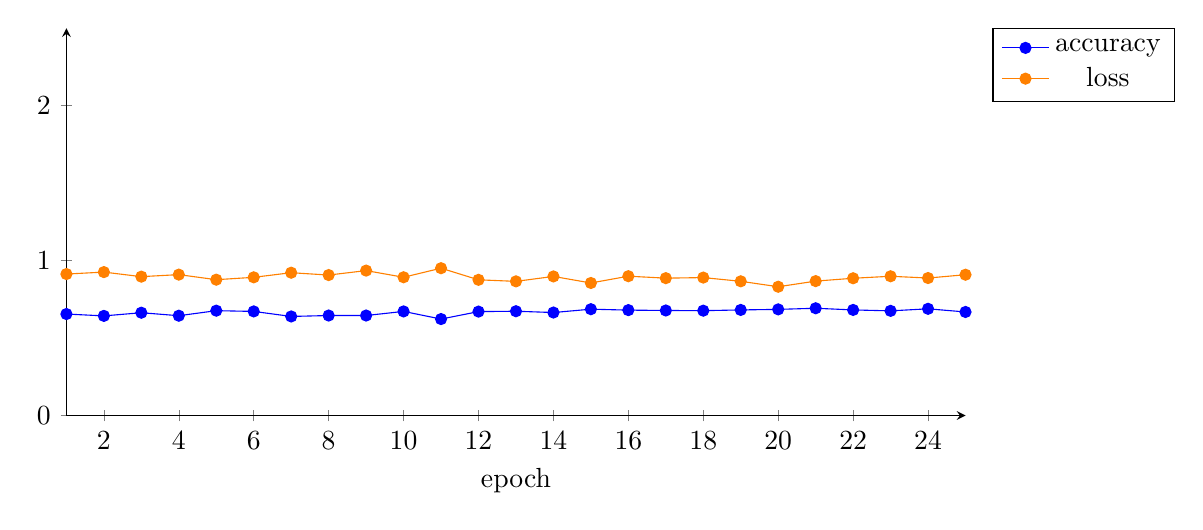
\begin{tikzpicture}
      \begin{axis}[
          width=13cm, height=6.5cm,
          ymin=0, ymax=2.5,
          xmin=1, xmax=25,
          axis x line=bottom,
          axis y line=left,
          xlabel=epoch,
          title={},
          axis on top=true, clip=false,
          legend pos=outer north east
      ]
      \addplot[mark=*, blue] coordinates {
          (1, 0.6550) (2, 0.6430) (3, 0.6635) (4, 0.6442) (5, 0.6767) (6, 0.6719) (7, 0.6394) (8, 0.6454) (9, 0.6454) (10, 0.6719) (11, 0.6226) (12, 0.6707) (13, 0.6731) (14, 0.6647) (15, 0.6863) (16, 0.6803) (17, 0.6779) (18, 0.6767) (19, 0.6815) (20, 0.6851) (21, 0.6923) (22, 0.6815) (23, 0.6755) (24, 0.6887) (25, 0.6683)
      };
      \addplot[mark=*, orange] coordinates {
          (1, 0.9131) (2, 0.9257) (3, 0.8963) (4, 0.9094) (5, 0.8767) (6, 0.8920) (7, 0.9218) (8, 0.9066) (9, 0.9354) (10, 0.8924) (11, 0.9509) (12, 0.8759) (13, 0.8659) (14, 0.8978) (15, 0.8555) (16, 0.8993) (17, 0.8866) (18, 0.8903) (19, 0.8663) (20, 0.8312) (21, 0.8675) (22, 0.8860) (23, 0.8988) (24, 0.8874) (25, 0.9088)
      };
      \addlegendentry{accuracy}
      \addlegendentry{loss}
      \end{axis}
  \end{tikzpicture}
\end{figure}
\bigskip

\clearpage
Test set performance:
\begin{itemize}
    \item Loss: 0.912283;
    \item Accuracy: 0.679087;
\end{itemize}
Already with LeNet we do not have bad performance both in terms of accuracy and loss. Looking at the confusion matrix this network seems to be quite accurate on the haze and sunny classes compared to the other two. We tries to do better switching to AlexNet.

\subsection{AlexNet}
AlexNet is much larger than LeNet, in fact it consists of 5 Convolutional Layers and 3 Dense Layers. There are more convolutional kernels that extract features in the images.
The first two convolutional levels are followed by the Max Pooling levels. The third, fourth and fifth convolutional layer are connected directly. The fifth conv is followed by a Max Pooling layer, whose output is divided into a series of two dense levels. The last dense level fits into a softmax classifier. The activation function used for all layers is ReLu, only the last dense layer use softmax classifier.

\bigskip
\begin{tabular}{|ll|r|}
  \hline
  {\bf Input Shape} & & 118 x 224         \\ \hline
  {\bf Total Params} & & 28.083.756       \\ \hline
  {\bf Trainable params} & & 28.062.620   \\ \hline
  {\bf Non trainable params} & & 21.136   \\ \hline
\end{tabular}

\bigskip
Test set performance:
\begin{itemize}
    \item Loss: 1.742811;
    \item Accuracy: 0.634615;
\end{itemize}

AlexNet seems worse than LeNet. This probably means that the {\em AveragePooling} is a better choiche than the {\em MaxPooling} for this type of dataset. The most common mistake of this network is to predict a rainy image as a snowy image. Obviously increasing the epochs we would have good results in the train set, close to $90\%$, but this does not happen for the performance in the test set and for this reason we stop the train at the $60^{th}$ epoch.

\begin{figure}[ht!]
  \caption{{\bf AlexNet $-$ Accuracy and Loss results in test set}}
  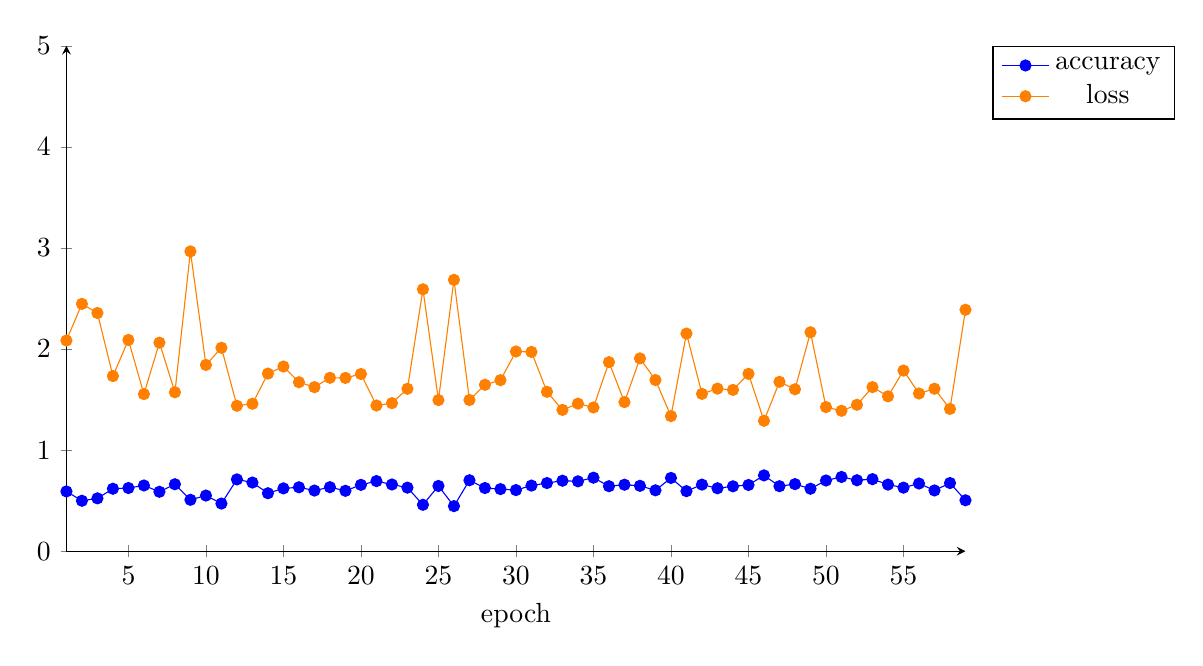
\begin{tikzpicture}
      \begin{axis}[
          width=13cm, height=8cm,
          ymin=0, ymax=5,
          xmin=1, xmax=59,
          axis x line=bottom,
          axis y line=left,
          xlabel=epoch,
          title={},
          axis on top=true, clip=false,
          legend pos=outer north east
      ]
      \addplot[mark=*, blue] coordinates {
          (1, 0.5913) (2, 0.4988) (3, 0.5228) (4, 0.6178) (5, 0.6250) (6, 0.6502) (7, 0.5877) (8, 0.6623) (9, 0.5084) (10, 0.5505) (11, 0.4712) (12, 0.7103) (13, 0.6791) (14, 0.5733) (15, 0.6214) (16, 0.6322) (17, 0.5998) (18, 0.6334) (19, 0.5974) (20, 0.6562) (21, 0.6935) (22, 0.6599) (23, 0.6286) (24, 0.4591) (25, 0.6454) (26, 0.4459) (27, 0.7019) (28, 0.6250) (29, 0.6142) (30, 0.6046) (31, 0.6490) (32, 0.6743) (33, 0.6971) (34, 0.6911) (35, 0.7272) (36, 0.6430) (37, 0.6575) (38, 0.6466) (39, 0.6022) (40, 0.7248) (41, 0.5938) (42, 0.6587) (43, 0.6226) (44, 0.6418) (45, 0.6550) (46, 0.7500) (47, 0.6430) (48, 0.6635) (49, 0.6178) (50, 0.6995) (51, 0.7344) (52, 0.7019) (53, 0.7127) (54, 0.6587) (55, 0.6286) (56, 0.6695) (57, 0.6010) (58, 0.6743) (59, 0.5036)
      };
      \addplot[mark=*, orange] coordinates {
          (1, 2.0844) (2, 2.4469) (3, 2.3562) (4, 1.7324) (5, 2.0902) (6, 1.5539) (7, 2.0631) (8, 1.5723) (9, 2.9661) (10, 1.8427) (11, 2.0123) (12, 1.4388) (13, 1.4587) (14, 1.7570) (15, 1.8272) (16, 1.6718) (17, 1.6228) (18, 1.7154) (19, 1.7144) (20, 1.7530) (21, 1.4414) (22, 1.4648) (23, 1.6069) (24, 2.5910) (25, 1.4948) (26, 2.6846) (27, 1.4959) (28, 1.6464) (29, 1.6923) (30, 1.9756) (31, 1.9715) (32, 1.5768) (33, 1.3977) (34, 1.4601) (35, 1.4221) (36, 1.8702) (37, 1.4749) (38, 1.9076) (39, 1.6934) (40, 1.3363) (41, 2.1531) (42, 1.5565) (43, 1.6083) (44, 1.5957) (45, 1.7548) (46, 1.2900) (47, 1.6756) (48, 1.6018) (49, 2.1659) (50, 1.4258) (51, 1.3889) (52, 1.4483) (53, 1.6232) (54, 1.5321) (55, 1.7871) (56, 1.5599) (57, 1.6072) (58, 1.4075) (59, 2.3886)
      };
      \addlegendentry{accuracy}
      \addlegendentry{loss}
      \end{axis}
  \end{tikzpicture}
\end{figure}
\bigskip

We stop here our experiments with well known networks because the most recent are too complex and in the next section we will try to use neural networks created from scratch.

\newpage
\section{My Neural Networks}
In this section we will see two neural networks created by me. What we will see is the improvement of the performance with very simple networks.
\subsection{ValerioNet 1}
ValerioNet 1 is a very simple convolutional neural network. It has two Convolution layers each of which is followed by an (2x2) AveragePooling level. The output is then passed to a Flatten layer and then to two Dense layers among which we have a level of Dropout to reduce overfitting. The activation function used is ReLu. In the two Conv layers we use two different kernel, the first have a size of (5x5) and the second of (3x3). We use also a padding value setted to {\em same}.

\bigskip
\begin{tabular}{|ll|r|}
  \hline
  {\bf Input Shape} & & 200 x 200         \\ \hline
  {\bf Total Params} & & 16.021.432       \\ \hline
  {\bf Trainable params} & & 16.021.43    \\ \hline
  {\bf Non trainable params} & & 0        \\ \hline
\end{tabular}

\bigskip
\begin{figure}[hbt!]
  \caption{{\bf ValerioNet1 $-$ Accuracy results}}
  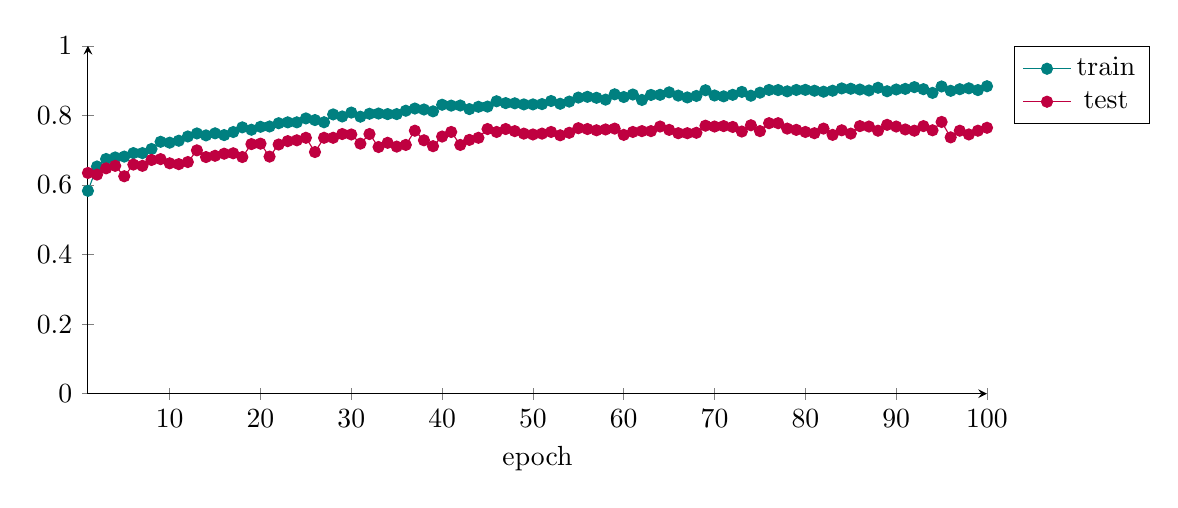
\begin{tikzpicture}
      \begin{axis}[
          width=13cm, height=6cm,
          ymin=0, ymax=1,
          xmin=1, xmax=100,
          axis x line=bottom,
          axis y line=left,
          xlabel=epoch,
          title={},
          axis on top=true, clip=false,
          legend pos=outer north east
      ]
      \addplot[mark=*, teal] coordinates {
          (1, 0.5831) (2, 0.6531) (3, 0.6747) (4, 0.6791) (5, 0.6816) (6, 0.6916) (7, 0.6916) (8, 0.7034) (9, 0.7241) (10, 0.7216) (11, 0.7272) (12, 0.7394) (13, 0.7481) (14, 0.7425) (15, 0.7484) (16, 0.7434) (17, 0.7522) (18, 0.7656) (19, 0.7588) (20, 0.7672) (21, 0.7681) (22, 0.7775) (23, 0.7800) (24, 0.7800) (25, 0.7913) (26, 0.7866) (27, 0.7803) (28, 0.8028) (29, 0.7969) (30, 0.8081) (31, 0.7963) (32, 0.8047) (33, 0.8053) (34, 0.8037) (35, 0.8037) (36, 0.8134) (37, 0.8197) (38, 0.8169) (39, 0.8116) (40, 0.8306) (41, 0.8281) (42, 0.8284) (43, 0.8181) (44, 0.8247) (45, 0.8253) (46, 0.8406) (47, 0.8353) (48, 0.8347) (49, 0.8316) (50, 0.8316) (51, 0.8325) (52, 0.8413) (53, 0.8334) (54, 0.8397) (55, 0.8512) (56, 0.8534) (57, 0.8506) (58, 0.8453) (59, 0.8606) (60, 0.8528) (61, 0.8600) (62, 0.8444) (63, 0.8588) (64, 0.8591) (65, 0.8662) (66, 0.8569) (67, 0.8516) (68, 0.8559) (69, 0.8722) (70, 0.8572) (71, 0.8547) (72, 0.8591) (73, 0.8675) (74, 0.8566) (75, 0.8653) (76, 0.8731) (77, 0.8728) (78, 0.8691) (79, 0.8731) (80, 0.8734) (81, 0.8709) (82, 0.8681) (83, 0.8709) (84, 0.8775) (85, 0.8766) (86, 0.8744) (87, 0.8716) (88, 0.8794) (89, 0.8694) (90, 0.8744) (91, 0.8762) (92, 0.8812) (93, 0.8753) (94, 0.8647) (95, 0.8831) (96, 0.8706) (97, 0.8753) (98, 0.8778) (99, 0.8728) (100, 0.8838)
      };
      \addplot[mark=*, purple] coordinates {
        (1, 0.6346) (2, 0.6298) (3, 0.6478) (4, 0.6550) (5, 0.6250) (6, 0.6587) (7, 0.6550) (8, 0.6719) (9, 0.6743) (10, 0.6623) (11, 0.6599) (12, 0.6659) (13, 0.6995) (14, 0.6803) (15, 0.6839) (16, 0.6899) (17, 0.6911) (18, 0.6803) (19, 0.7175) (20, 0.7188) (21, 0.6815) (22, 0.7163) (23, 0.7260) (24, 0.7284) (25, 0.7356) (26, 0.6947) (27, 0.7356) (28, 0.7356) (29, 0.7464) (30, 0.7452) (31, 0.7188) (32, 0.7464) (33, 0.7091) (34, 0.7212) (35, 0.7103) (36, 0.7151) (37, 0.7560) (38, 0.7284) (39, 0.7115) (40, 0.7392) (41, 0.7524) (42, 0.7151) (43, 0.7296) (44, 0.7356) (45, 0.7608) (46, 0.7524) (47, 0.7608) (48, 0.7548) (49, 0.7476) (50, 0.7452) (51, 0.7476) (52, 0.7524) (53, 0.7428) (54, 0.7500) (55, 0.7632) (56, 0.7608) (57, 0.7572) (58, 0.7596) (59, 0.7620) (60, 0.7440) (61, 0.7524) (62, 0.7548) (63, 0.7548) (64, 0.7680) (65, 0.7584) (66, 0.7488) (67, 0.7488) (68, 0.7500) (69, 0.7704) (70, 0.7680) (71, 0.7692) (72, 0.7668) (73, 0.7536) (74, 0.7716) (75, 0.7548) (76, 0.7776) (77, 0.7776) (78, 0.7620) (79, 0.7584) (80, 0.7524) (81, 0.7488) (82, 0.7620) (83, 0.7440) (84, 0.7572) (85, 0.7476) (86, 0.7692) (87, 0.7680) (88, 0.7560) (89, 0.7728) (90, 0.7680) (91, 0.7596) (92, 0.7560) (93, 0.7692) (94, 0.7572) (95, 0.7812) (96, 0.7368) (97, 0.7560) (98, 0.7452) (99, 0.7560) (100, 0.7644)
      };
      \addlegendentry{train}
      \addlegendentry{test}
      \end{axis}
  \end{tikzpicture}
\end{figure}

\begin{figure}[hbt!]
  \caption{{\bf ValerioNet1 $-$ Loss results}}
  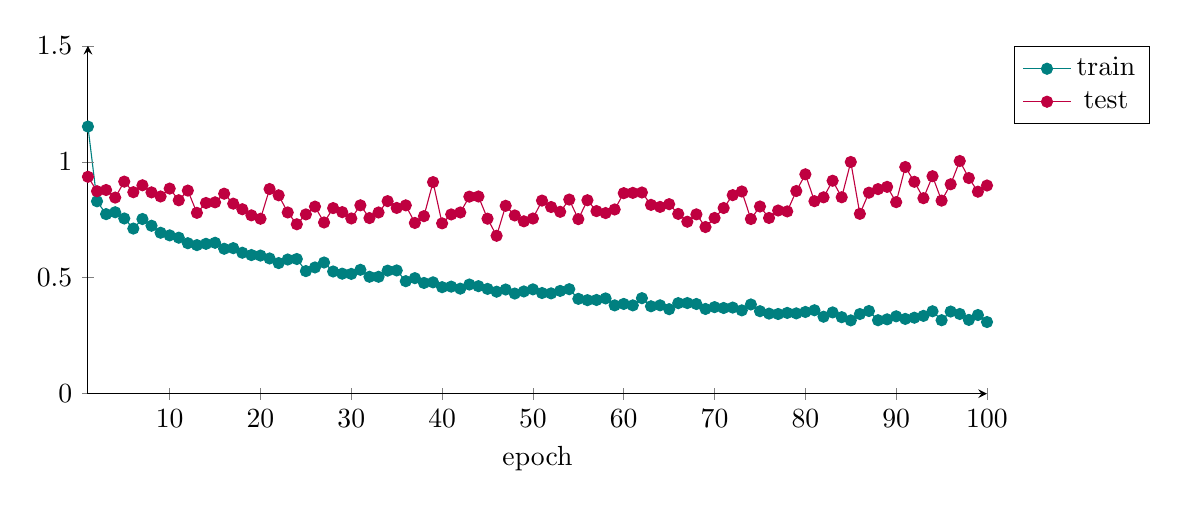
\begin{tikzpicture}
      \begin{axis}[
          width=13cm, height=6cm,
          ymin=0, ymax=1.5,
          xmin=1, xmax=100,
          axis x line=bottom,
          axis y line=left,
          xlabel=epoch,
          title={},
          axis on top=true, clip=false,
          legend pos=outer north east
      ]
      \addplot[mark=*, teal] coordinates {
        (1, 1.1519) (2, 0.8297) (3, 0.7743) (4, 0.7824) (5, 0.7556) (6, 0.7120) (7, 0.7532) (8, 0.7242) (9, 0.6940) (10, 0.6827) (11, 0.6727) (12, 0.6489) (13, 0.6407) (14, 0.6462) (15, 0.6507) (16, 0.6250) (17, 0.6276) (18, 0.6078) (19, 0.5978) (20, 0.5956) (21, 0.5832) (22, 0.5632) (23, 0.5786) (24, 0.5808) (25, 0.5287) (26, 0.5444) (27, 0.5657) (28, 0.5270) (29, 0.5176) (30, 0.5166) (31, 0.5342) (32, 0.5042) (33, 0.5041) (34, 0.5306) (35, 0.5316) (36, 0.4852) (37, 0.4983) (38, 0.4776) (39, 0.4802) (40, 0.4594) (41, 0.4617) (42, 0.4530) (43, 0.4708) (44, 0.4637) (45, 0.4520) (46, 0.4399) (47, 0.4493) (48, 0.4319) (49, 0.4409) (50, 0.4499) (51, 0.4342) (52, 0.4326) (53, 0.4433) (54, 0.4507) (55, 0.4090) (56, 0.4034) (57, 0.4042) (58, 0.4109) (59, 0.3809) (60, 0.3871) (61, 0.3809) (62, 0.4119) (63, 0.3770) (64, 0.3811) (65, 0.3645) (66, 0.3906) (67, 0.3909) (68, 0.3868) (69, 0.3655) (70, 0.3733) (71, 0.3696) (72, 0.3714) (73, 0.3594) (74, 0.3848) (75, 0.3558) (76, 0.3454) (77, 0.3437) (78, 0.3484) (79, 0.3464) (80, 0.3525) (81, 0.3598) (82, 0.3320) (83, 0.3506) (84, 0.3300) (85, 0.3162) (86, 0.3436) (87, 0.3566) (88, 0.3169) (89, 0.3206) (90, 0.3337) (91, 0.3226) (92, 0.3277) (93, 0.3356) (94, 0.3554) (95, 0.3169) (96, 0.3543) (97, 0.3438) (98, 0.3183) (99, 0.3393) (100, 0.3091)
      };
      \addplot[mark=*, purple] coordinates {
        (1, 0.9353) (2, 0.8731) (3, 0.8783) (4, 0.8456) (5, 0.9144) (6, 0.8689) (7, 0.8987) (8, 0.8681) (9, 0.8504) (10, 0.8844) (11, 0.8341) (12, 0.8758) (13, 0.7798) (14, 0.8224) (15, 0.8251) (16, 0.8624) (17, 0.8194) (18, 0.7954) (19, 0.7690) (20, 0.7543) (21, 0.8825) (22, 0.8555) (23, 0.7815) (24, 0.7306) (25, 0.7731) (26, 0.8067) (27, 0.7383) (28, 0.8003) (29, 0.7829) (30, 0.7556) (31, 0.8123) (32, 0.7573) (33, 0.7814) (34, 0.8303) (35, 0.8010) (36, 0.8121) (37, 0.7363) (38, 0.7655) (39, 0.9123) (40, 0.7345) (41, 0.7730) (42, 0.7814) (43, 0.8497) (44, 0.8504) (45, 0.7546) (46, 0.6809) (47, 0.8102) (48, 0.7686) (49, 0.7433) (50, 0.7553) (51, 0.8327) (52, 0.8050) (53, 0.7842) (54, 0.8371) (55, 0.7527) (56, 0.8342) (57, 0.7873) (58, 0.7789) (59, 0.7943) (60, 0.8647) (61, 0.8659) (62, 0.8676) (63, 0.8142) (64, 0.8055) (65, 0.8172) (66, 0.7753) (67, 0.7416) (68, 0.7733) (69, 0.7187) (70, 0.7577) (71, 0.8006) (72, 0.8562) (73, 0.8719) (74, 0.7532) (75, 0.8072) (76, 0.7578) (77, 0.7899) (78, 0.7861) (79, 0.8739) (80, 0.9460) (81, 0.8301) (82, 0.8467) (83, 0.9182) (84, 0.8470) (85, 0.9991) (86, 0.7755) (87, 0.8668) (88, 0.8821) (89, 0.8918) (90, 0.8260) (91, 0.9774) (92, 0.9137) (93, 0.8430) (94, 0.9378) (95, 0.8325) (96, 0.9030) (97, 1.0033) (98, 0.9298) (99, 0.8710) (100, 0.8977)
      };
      \addlegendentry{train}
      \addlegendentry{test}
      \end{axis}
  \end{tikzpicture}
\end{figure}
\bigskip

\newpage
Test set performance:
\begin{itemize}
    \item Loss: 0.870954;
    \item Accuracy: 0.769231;
\end{itemize}

Oh well this results are very nice than those seen before. My net is better than AlexNet and LeNet, this means that i won (:D). But analyze the results. In the following figure we see the confusion matrix and the value of precision and recall:\newline \newline
\begin{minipage}[c]{.5\textwidth}
   \centering
   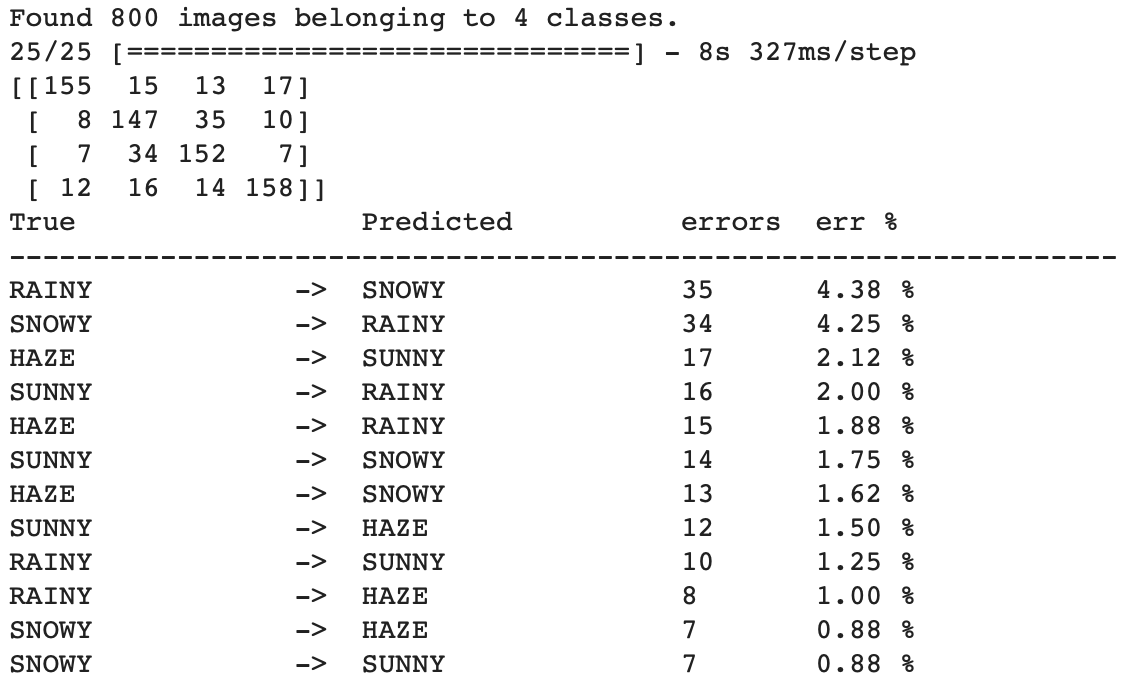
\includegraphics[width=\textwidth]{pic1}
\end{minipage}
\hspace{1em}
\begin{minipage}[c]{.5\textwidth}
   \centering
   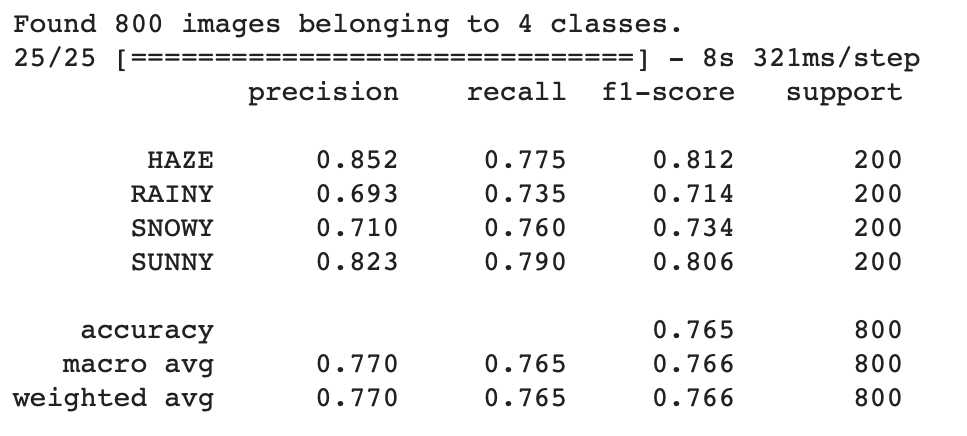
\includegraphics[width=\textwidth]{pic2.png}
\end{minipage}

\bigskip
As we can see from the images, this networks has nice results but also in this case the most common error is the misclassification of the rainy with snowy. This network is very simple and not very deeper, generally two hidden layers are enough but in theory a deeper network is better because it needs less neurons to reach the results like two hidden layers. For this reason in the following section we try to make ValerioNet1 deeper and we compare the results.

\subsection{ValerioNet 2}
ValerioNet 2 is deeper than the previous version. It is a mix between the three networks seen before. In fact it has 5 Convolutional layers, the first two use {\em tanh} activation function and a (5x5) kernel, like LeNet layers, and they are followed by an (2x2) AveragePooling level. The next three Conv layers are like AlexNet, in fact the $3^{rd}$, $4^{th}$ and the $5^{th}$ are followed by a Batch Normalization layer and use ReLu activation function, with (3x3) kernels. The output is then passed to a Flatten layer and then to two Dense layers among which we have a level of Dropout and other two levels of Batch Normalization, to reduce overfitting. The last Dense layer uses softmax classifier. The optimizer used is {\em adam}. Complete structure is the following:

\bigskip
\begin{minipage}[c]{.5\textwidth}
   \centering
   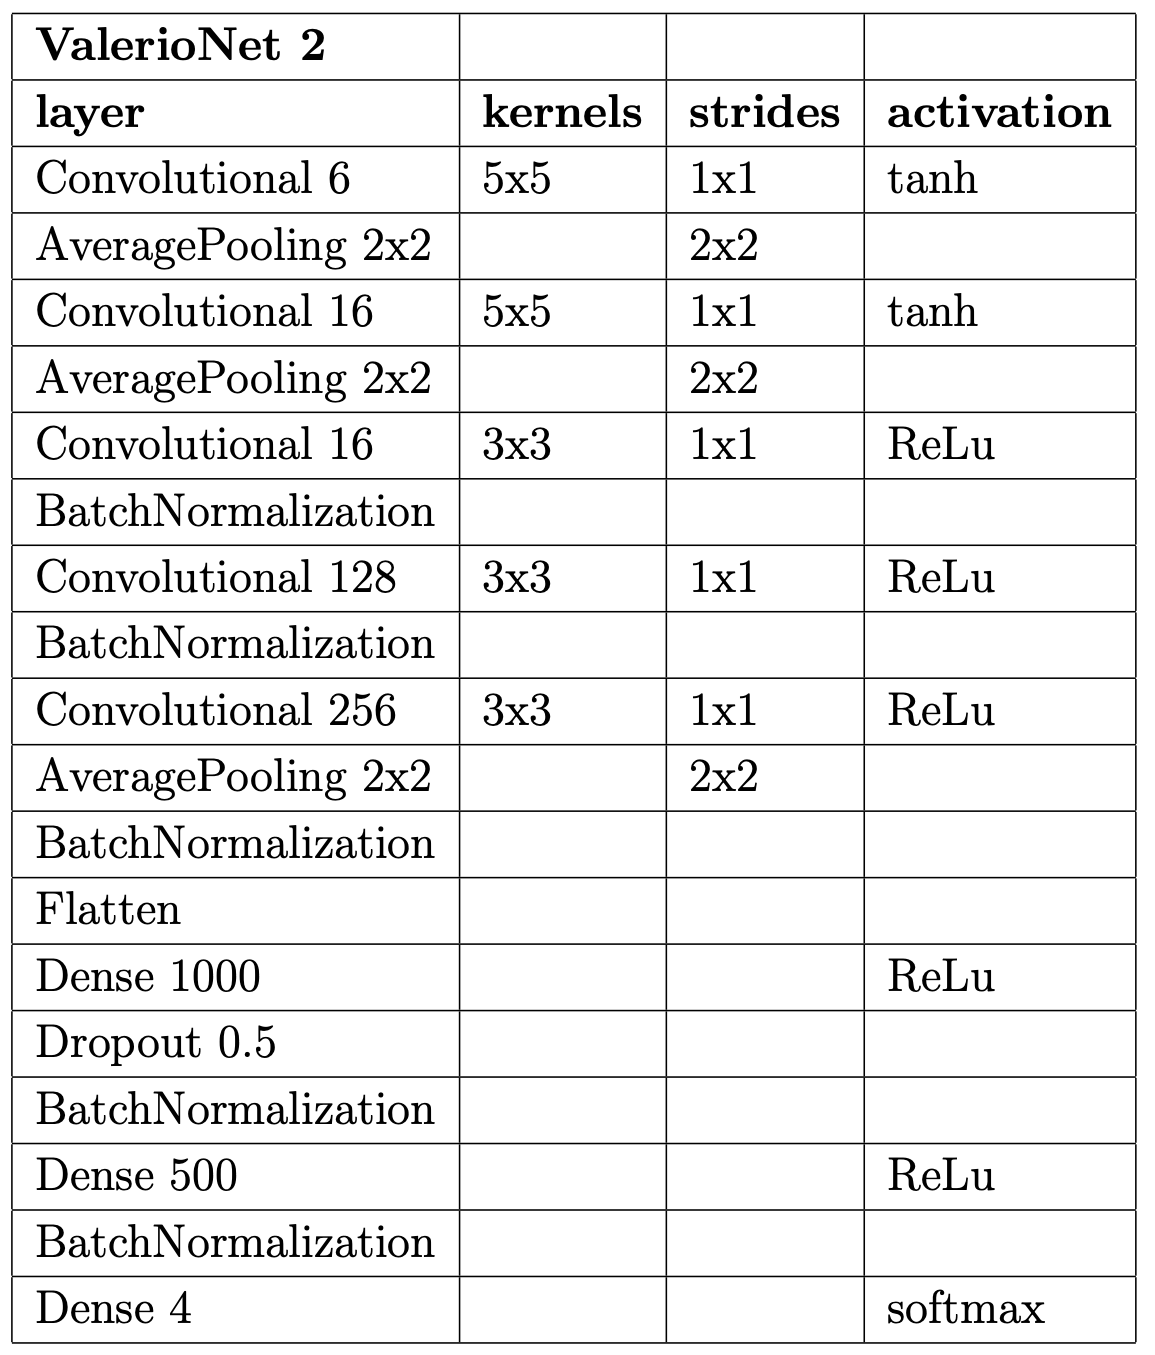
\includegraphics[width=\textwidth]{pic3}
\end{minipage}
\bigskip

\bigskip
\begin{tabular}{|ll|r|}
  \hline
  {\bf Input Shape} & & 200 x 200         \\ \hline
  {\bf Total Params} & & 113.726.024       \\ \hline
  {\bf Trainable params} & & 113.722.224    \\ \hline
  {\bf Non trainable params} & & 3.800        \\ \hline
\end{tabular}

\bigskip
\begin{figure}[hbt!]
  \caption{{\bf ValerioNet2 $-$ Accuracy results}}
  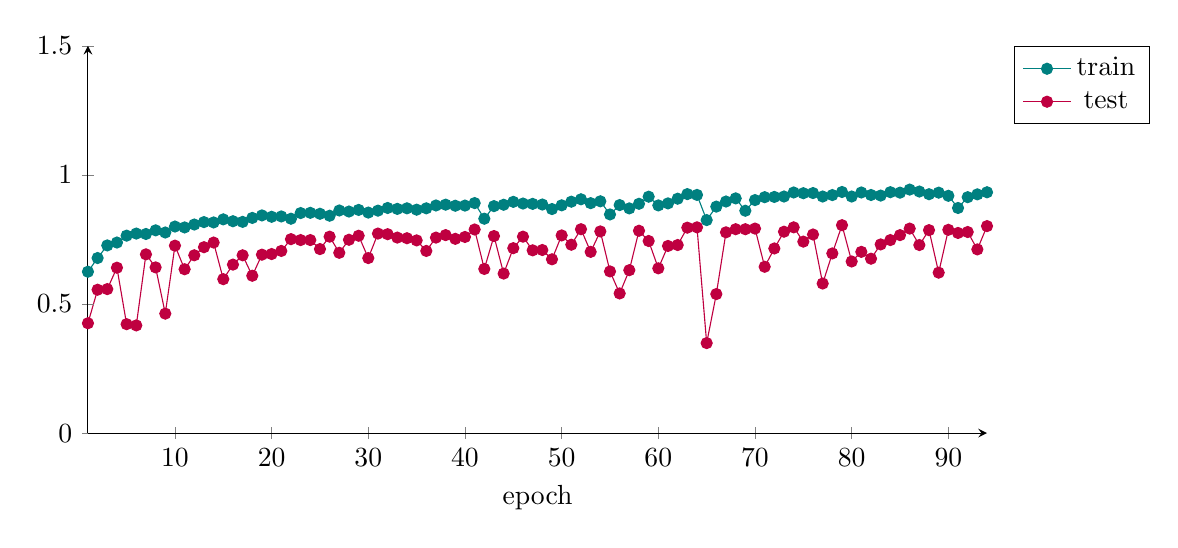
\begin{tikzpicture}
      \begin{axis}[
          width=13cm, height=6.5cm,
          ymin=0, ymax=1.5,
          xmin=1, xmax=94,
          axis x line=bottom,
          axis y line=left,
          xlabel=epoch,
          title={},
          axis on top=true, clip=false,
          legend pos=outer north east
      ]
      \addplot[mark=*, teal] coordinates {
        (1, 0.6250) (2, 0.6781) (3, 0.7269) (4, 0.7381) (5, 0.7647) (6, 0.7728) (7, 0.7712) (8, 0.7853) (9, 0.7769) (10, 0.8000) (11, 0.7966) (12, 0.8078) (13, 0.8172) (14, 0.8159) (15, 0.8278) (16, 0.8206) (17, 0.8181) (18, 0.8334) (19, 0.8431) (20, 0.8378) (21, 0.8391) (22, 0.8303) (23, 0.8522) (24, 0.8531) (25, 0.8494) (26, 0.8419) (27, 0.8622) (28, 0.8581) (29, 0.8644) (30, 0.8541) (31, 0.8616) (32, 0.8719) (33, 0.8684) (34, 0.8706) (35, 0.8653) (36, 0.8706) (37, 0.8816) (38, 0.8847) (39, 0.8806) (40, 0.8812) (41, 0.8909) (42, 0.8303) (43, 0.8791) (44, 0.8844) (45, 0.8956) (46, 0.8891) (47, 0.8878) (48, 0.8853) (49, 0.8678) (50, 0.8822) (51, 0.8962) (52, 0.9056) (53, 0.8906) (54, 0.8978) (55, 0.8469) (56, 0.8831) (57, 0.8703) (58, 0.8881) (59, 0.9156) (60, 0.8819) (61, 0.8897) (62, 0.9078) (63, 0.9256) (64, 0.9225) (65, 0.8250) (66, 0.8772) (67, 0.8969) (68, 0.9091) (69, 0.8612) (70, 0.9025) (71, 0.9137) (72, 0.9147) (73, 0.9163) (74, 0.9319) (75, 0.9291) (76, 0.9297) (77, 0.9163) (78, 0.9219) (79, 0.9338) (80, 0.9163) (81, 0.9319) (82, 0.9222) (83, 0.9200) (84, 0.9331) (85, 0.9313) (86, 0.9431) (87, 0.9356) (88, 0.9253) (89, 0.9313) (90, 0.9191) (91, 0.8719) (92, 0.9137) (93, 0.9247) (94, 0.9328)
      };
      \addplot[mark=*, purple] coordinates {
        (1, 0.4255) (2, 0.5553) (3, 0.5577) (4, 0.6406) (5, 0.4219) (6, 0.4171) (7, 0.6923) (8, 0.6418) (9, 0.4627) (10, 0.7260) (11, 0.6346) (12, 0.6887) (13, 0.7200) (14, 0.7380) (15, 0.5962) (16, 0.6526) (17, 0.6887) (18, 0.6094) (19, 0.6911) (20, 0.6935) (21, 0.7055) (22, 0.7512) (23, 0.7476) (24, 0.7476) (25, 0.7127) (26, 0.7608) (27, 0.6983) (28, 0.7488) (29, 0.7644) (30, 0.6779) (31, 0.7728) (32, 0.7704) (33, 0.7572) (34, 0.7548) (35, 0.7464) (36, 0.7055) (37, 0.7572) (38, 0.7668) (39, 0.7524) (40, 0.7596) (41, 0.7885) (42, 0.6358) (43, 0.7632) (44, 0.6178) (45, 0.7163) (46, 0.7608) (47, 0.7079) (48, 0.7091) (49, 0.6731) (50, 0.7656) (51, 0.7296) (52, 0.7897) (53, 0.7019) (54, 0.7812) (55, 0.6262) (56, 0.5409) (57, 0.6310) (58, 0.7837) (59, 0.7440) (60, 0.6382) (61, 0.7248) (62, 0.7284) (63, 0.7957) (64, 0.7969) (65, 0.3486) (66, 0.5385) (67, 0.7776) (68, 0.7897) (69, 0.7897) (70, 0.7921) (71, 0.6442) (72, 0.7151) (73, 0.7800) (74, 0.7969) (75, 0.7416) (76, 0.7692) (77, 0.5793) (78, 0.6959) (79, 0.8053) (80, 0.6647) (81, 0.7019) (82, 0.6755) (83, 0.7308) (84, 0.7476) (85, 0.7668) (86, 0.7921) (87, 0.7284) (88, 0.7861) (89, 0.6214) (90, 0.7873) (91, 0.7752) (92, 0.7788) (93, 0.7115) (94, 0.8017)
      };
      \addlegendentry{train}
      \addlegendentry{test}
      \end{axis}
  \end{tikzpicture}
\end{figure}

\bigskip
\begin{figure}[hbt!]
  \caption{{\bf ValerioNet2 $-$ Loss results}}
  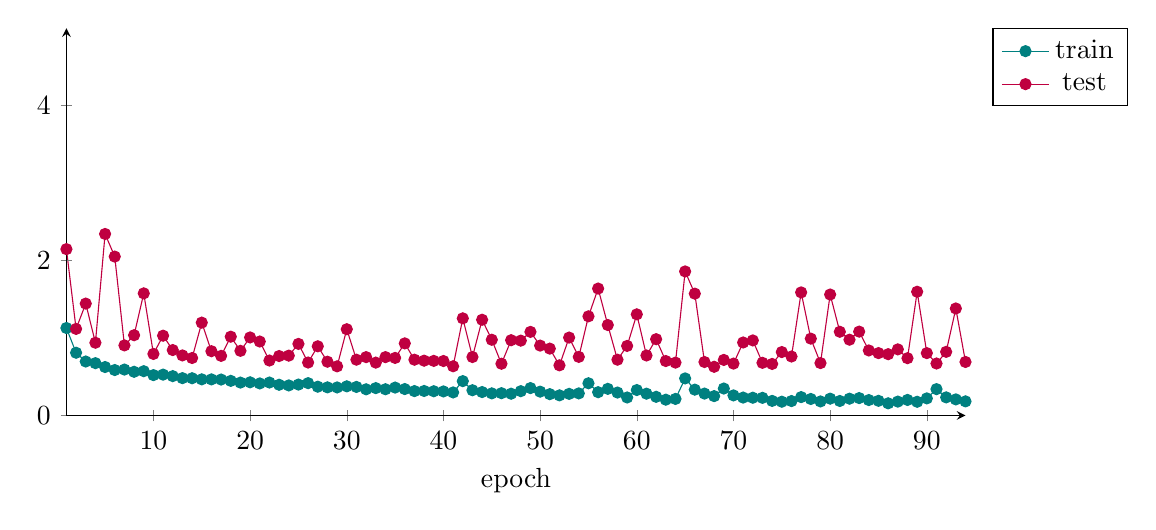
\begin{tikzpicture}
      \begin{axis}[
          width=13cm, height=6.5cm,
          ymin=0, ymax=5,
          xmin=1, xmax=94,
          axis x line=bottom,
          axis y line=left,
          xlabel=epoch,
          title={},
          axis on top=true, clip=false,
          legend pos=outer north east
      ]
      \addplot[mark=*, teal] coordinates {
        (1, 1.1295) (2, 0.8101) (3, 0.6969) (4, 0.6758) (5, 0.6258) (6, 0.5870) (7, 0.5928) (8, 0.5641) (9, 0.5721) (10, 0.5214) (11, 0.5276) (12, 0.5083) (13, 0.4823) (14, 0.4812) (15, 0.4669) (16, 0.4663) (17, 0.4642) (18, 0.4471) (19, 0.4248) (20, 0.4286) (21, 0.4140) (22, 0.4255) (23, 0.3966) (24, 0.3883) (25, 0.3992) (26, 0.4176) (27, 0.3719) (28, 0.3633) (29, 0.3622) (30, 0.3765) (31, 0.3688) (32, 0.3382) (33, 0.3536) (34, 0.3390) (35, 0.3605) (36, 0.3413) (37, 0.3151) (38, 0.3166) (39, 0.3132) (40, 0.3108) (41, 0.2979) (42, 0.4438) (43, 0.3263) (44, 0.3027) (45, 0.2859) (46, 0.2881) (47, 0.2812) (48, 0.3141) (49, 0.3539) (50, 0.3079) (51, 0.2755) (52, 0.2601) (53, 0.2792) (54, 0.2852) (55, 0.4162) (56, 0.3009) (57, 0.3440) (58, 0.2963) (59, 0.2326) (60, 0.3285) (61, 0.2816) (62, 0.2411) (63, 0.2041) (64, 0.2139) (65, 0.4788) (66, 0.3337) (67, 0.2828) (68, 0.2503) (69, 0.3481) (70, 0.2596) (71, 0.2314) (72, 0.2293) (73, 0.2280) (74, 0.1884) (75, 0.1779) (76, 0.1863) (77, 0.2374) (78, 0.2132) (79, 0.1816) (80, 0.2174) (81, 0.1875) (82, 0.2170) (83, 0.2248) (84, 0.1993) (85, 0.1896) (86, 0.1573) (87, 0.1793) (88, 0.2007) (89, 0.1771) (90, 0.2209) (91, 0.3403) (92, 0.2339) (93, 0.2079) (94, 0.1825)
      };
      \addplot[mark=*, purple] coordinates {
        (1, 2.1478) (2, 1.1179) (3, 1.4447) (4, 0.9393) (5, 2.3437) (6, 2.0515) (7, 0.9052) (8, 1.0368) (9, 1.5770) (10, 0.7950) (11, 1.0304) (12, 0.8448) (13, 0.7757) (14, 0.7422) (15, 1.1990) (16, 0.8300) (17, 0.7697) (18, 1.0175) (19, 0.8347) (20, 1.0077) (21, 0.9551) (22, 0.7095) (23, 0.7677) (24, 0.7728) (25, 0.9244) (26, 0.6838) (27, 0.8935) (28, 0.6943) (29, 0.6347) (30, 1.1139) (31, 0.7204) (32, 0.7536) (33, 0.6827) (34, 0.7537) (35, 0.7434) (36, 0.9311) (37, 0.7203) (38, 0.7078) (39, 0.7051) (40, 0.7032) (41, 0.6358) (42, 1.2544) (43, 0.7549) (44, 1.2361) (45, 0.9778) (46, 0.6682) (47, 0.9721) (48, 0.9665) (49, 1.0794) (50, 0.9026) (51, 0.8636) (52, 0.6477) (53, 1.0061) (54, 0.7565) (55, 1.2803) (56, 1.6389) (57, 1.1680) (58, 0.7203) (59, 0.8982) (60, 1.3061) (61, 0.7749) (62, 0.9854) (63, 0.7030) (64, 0.6827) (65, 1.8600) (66, 1.5730) (67, 0.6906) (68, 0.6288) (69, 0.7175) (70, 0.6699) (71, 0.9426) (72, 0.9692) (73, 0.6800) (74, 0.6657) (75, 0.8190) (76, 0.7615) (77, 1.5892) (78, 0.9922) (79, 0.6767) (80, 1.5619) (81, 1.0808) (82, 0.9786) (83, 1.0829) (84, 0.8396) (85, 0.8054) (86, 0.7916) (87, 0.8537) (88, 0.7399) (89, 1.5977) (90, 0.8054) (91, 0.6710) (92, 0.8217) (93, 1.3817) (94, 0.6913)
      };
      \addlegendentry{train}
      \addlegendentry{test}
      \end{axis}
  \end{tikzpicture}
\end{figure}

\newpage
Final epoch performance:
\begin{itemize}
    \item Loss: 0.1825;
    \item Accuracy: 0.9328;
\end{itemize}

Test set performance:
\begin{itemize}
    \item Loss: 0.691415;
    \item Accuracy: 0.801683;
\end{itemize}

Confusion matrix and score: \newline
\begin{minipage}[c]{.5\textwidth}
   \centering
   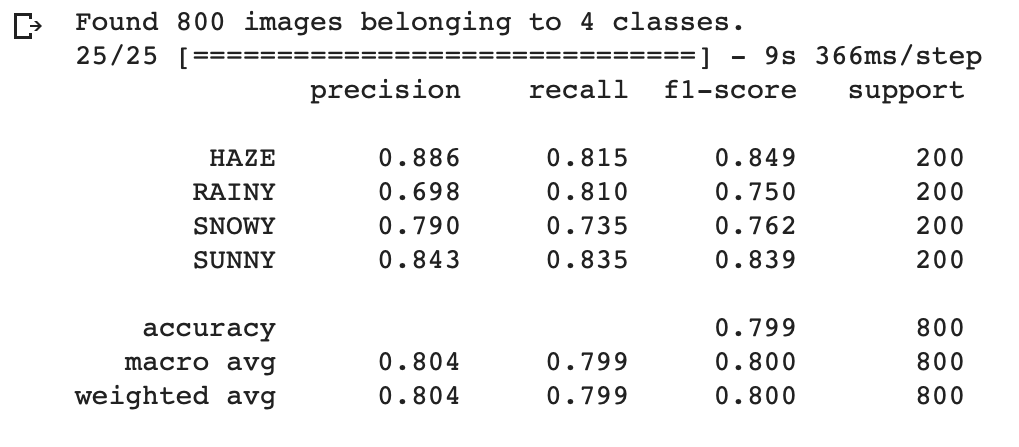
\includegraphics[width=\textwidth]{pic4}
\end{minipage}
\hspace{1em}
\begin{minipage}[c]{.5\textwidth}
   \centering
   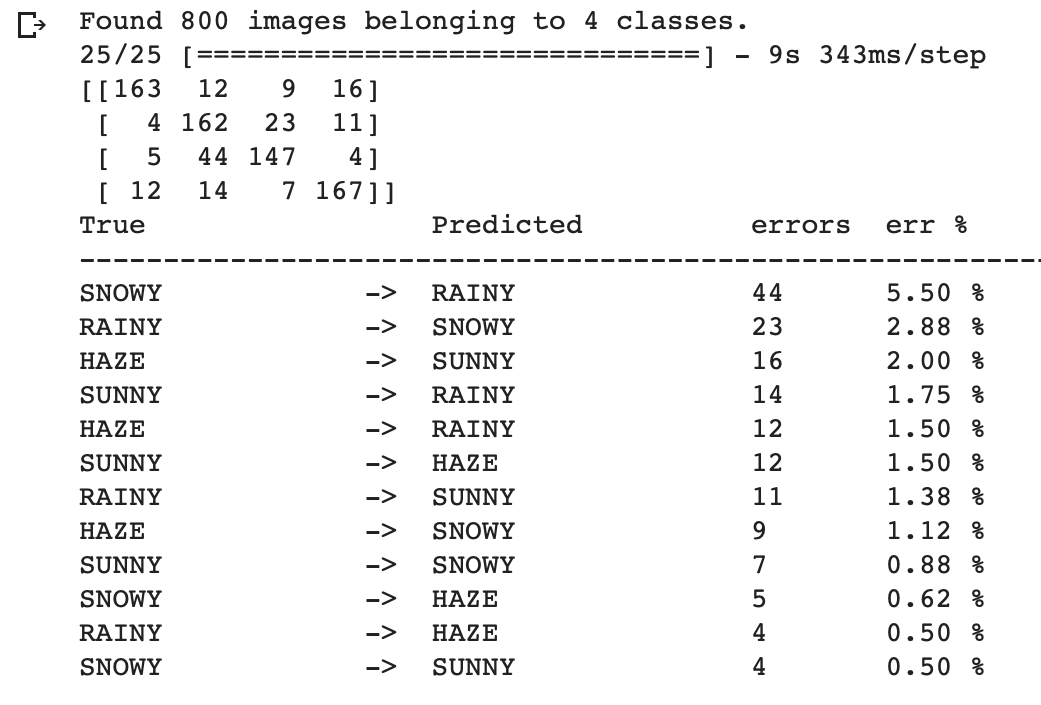
\includegraphics[width=\textwidth]{pic5}
\end{minipage}

Once again we have improved performance to a very good result. Looking at the confusion matrix, even with this network the problem is in the classification of the rainy images, but we improved the performance in the other classes specially for the haze class. The problem of this network is that, as we can see from the graphs, the results in the test set is a bit unstable. So we won't immediately discard ValerioNet1 because, even with slightly lower results, it is more stable and could be the best choice.

However, even trying to modify this network to increase performance, this is the best result we have been able to achieve. But this was predictable given the very small size of the dataset. For this reason we stop our analysis  with neural networks here and continue reporting some experiments with {\em Transfer Learning}.

\newpage
\section{Transfer Learning}
Transfer Learning is a Machine Learning technique based on which a model is trained and developed for an activity and is then reused in a second related activity. It refers to the situation in which what was learned in a setting is used to improve optimization in another setting. Transfer Learning allows us to start with the learned features on the dataset and adjust the structure of the model, instead of starting the learning process on the data from scratch with random weight initialization. It is usually applied when there is a small dataset.

In this homework we use Transfer Learning to improve the performances of ValerioNet1 and ValerioNet2.

\subsection{ValerioNet 1 - transfer model}

\bigskip
\begin{figure}[hbt!]
  \caption{{\bf ValerioNet1 Transfer $-$ Accuracy results}}
  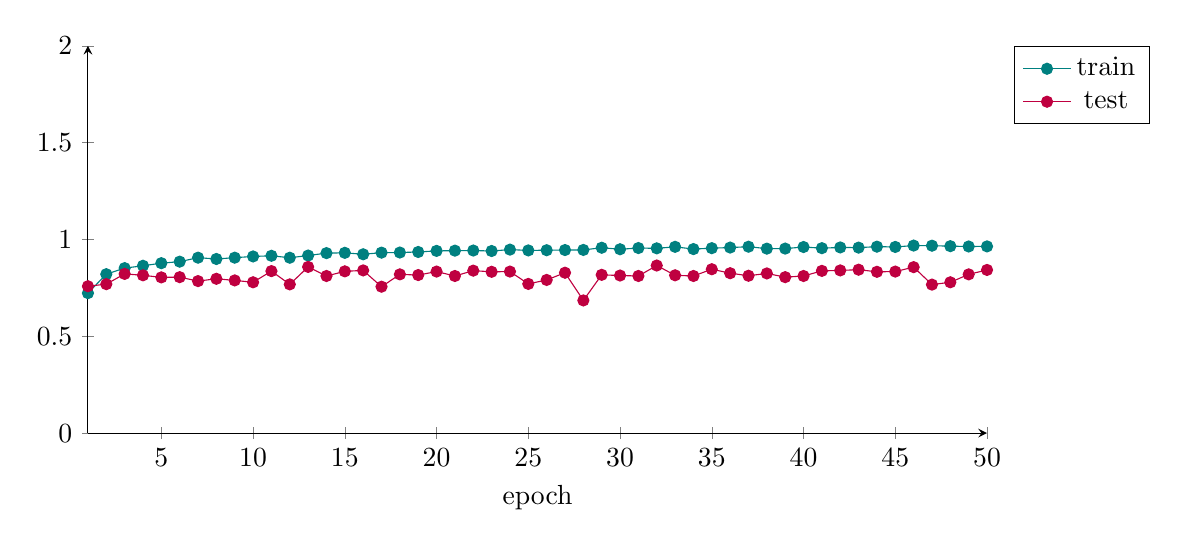
\begin{tikzpicture}
      \begin{axis}[
          width=13cm, height=6.5cm,
          ymin=0, ymax=2,
          xmin=1, xmax=50,
          axis x line=bottom,
          axis y line=left,
          xlabel=epoch,
          title={},
          axis on top=true, clip=false,
          legend pos=outer north east
      ]
      \addplot[mark=*, teal] coordinates {
        (1, 0.7228) (2, 0.8206) (3, 0.8519) (4, 0.8641) (5, 0.8775) (6, 0.8853) (7, 0.9059) (8, 0.8991) (9, 0.9059) (10, 0.9122) (11, 0.9156) (12, 0.9056) (13, 0.9169) (14, 0.9294) (15, 0.9309) (16, 0.9234) (17, 0.9319) (18, 0.9325) (19, 0.9353) (20, 0.9409) (21, 0.9422) (22, 0.9428) (23, 0.9403) (24, 0.9475) (25, 0.9434) (26, 0.9444) (27, 0.9453) (28, 0.9459) (29, 0.9572) (30, 0.9494) (31, 0.9556) (32, 0.9541) (33, 0.9619) (34, 0.9503) (35, 0.9550) (36, 0.9581) (37, 0.9625) (38, 0.9525) (39, 0.9528) (40, 0.9609) (41, 0.9550) (42, 0.9587) (43, 0.9578) (44, 0.9628) (45, 0.9613) (46, 0.9684) (47, 0.9678) (48, 0.9653) (49, 0.9637) (50, 0.9641)
      };
      \addplot[mark=*, purple] coordinates {
        (1, 0.7584) (2, 0.7692) (3, 0.8221) (4, 0.8149) (5, 0.8041) (6, 0.8053) (7, 0.7849) (8, 0.7969) (9, 0.7885) (10, 0.7788) (11, 0.8365) (12, 0.7680) (13, 0.8582) (14, 0.8113) (15, 0.8353) (16, 0.8401) (17, 0.7560) (18, 0.8197) (19, 0.8161) (20, 0.8341) (21, 0.8113) (22, 0.8389) (23, 0.8329) (24, 0.8341) (25, 0.7704) (26, 0.7909) (27, 0.8281) (28, 0.6851) (29, 0.8173) (30, 0.8137) (31, 0.8113) (32, 0.8654) (33, 0.8149) (34, 0.8113) (35, 0.8462) (36, 0.8257) (37, 0.8125) (38, 0.8245) (39, 0.8053) (40, 0.8113) (41, 0.8377) (42, 0.8401) (43, 0.8438) (44, 0.8329) (45, 0.8341) (46, 0.8570) (47, 0.7668) (48, 0.7788) (49, 0.8197) (50, 0.8425)
      };
      \addlegendentry{train}
      \addlegendentry{test}
      \end{axis}
  \end{tikzpicture}
\end{figure}

\bigskip
\begin{figure}[hbt!]
  \caption{{\bf ValerioNet1 Transfer $-$ Loss results}}
  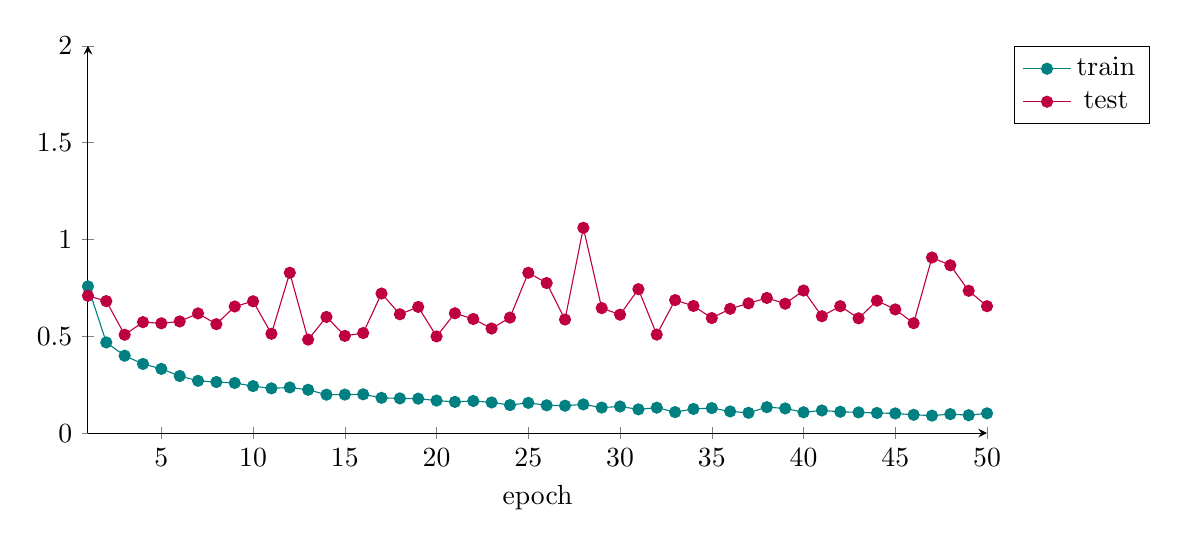
\begin{tikzpicture}
      \begin{axis}[
          width=13cm, height=6.5cm,
          ymin=0, ymax=2,
          xmin=1, xmax=50,
          axis x line=bottom,
          axis y line=left,
          xlabel=epoch,
          title={},
          axis on top=true, clip=false,
          legend pos=outer north east
      ]
      \addplot[mark=*, teal] coordinates {
        (1, 0.7578) (2, 0.4681) (3, 0.3996) (4, 0.3572) (5, 0.3317) (6, 0.2949) (7, 0.2699) (8, 0.2638) (9, 0.2587) (10, 0.2427) (11, 0.2310) (12, 0.2357) (13, 0.2237) (14, 0.1984) (15, 0.1988) (16, 0.2002) (17, 0.1821) (18, 0.1791) (19, 0.1778) (20, 0.1680) (21, 0.1611) (22, 0.1658) (23, 0.1583) (24, 0.1448) (25, 0.1561) (26, 0.1435) (27, 0.1415) (28, 0.1481) (29, 0.1317) (30, 0.1374) (31, 0.1226) (32, 0.1313) (33, 0.1083) (34, 0.1246) (35, 0.1293) (36, 0.1118) (37, 0.1047) (38, 0.1338) (39, 0.1274) (40, 0.1074) (41, 0.1168) (42, 0.1101) (43, 0.1069) (44, 0.1040) (45, 0.1016) (46, 0.0945) (47, 0.0903) (48, 0.0980) (49, 0.0923) (50, 0.1020)
      };
      \addplot[mark=*, purple] coordinates {
        (1, 0.7092) (2, 0.6815) (3, 0.5078) (4, 0.5729) (5, 0.5670) (6, 0.5765) (7, 0.6181) (8, 0.5626) (9, 0.6538) (10, 0.6807) (11, 0.5128) (12, 0.8280) (13, 0.4828) (14, 0.5998) (15, 0.5020) (16, 0.5167) (17, 0.7207) (18, 0.6137) (19, 0.6515) (20, 0.4992) (21, 0.6187) (22, 0.5893) (23, 0.5401) (24, 0.5965) (25, 0.8278) (26, 0.7749) (27, 0.5864) (28, 1.0603) (29, 0.6456) (30, 0.6115) (31, 0.7433) (32, 0.5086) (33, 0.6869) (34, 0.6566) (35, 0.5940) (36, 0.6418) (37, 0.6700) (38, 0.6980) (39, 0.6681) (40, 0.7361) (41, 0.6036) (42, 0.6555) (43, 0.5927) (44, 0.6840) (45, 0.6386) (46, 0.5675) (47, 0.9067) (48, 0.8666) (49, 0.7349) (50, 0.6554)
      };
      \addlegendentry{train}
      \addlegendentry{test}
      \end{axis}
  \end{tikzpicture}
\end{figure}

\newpage
Final epoch performance:
\begin{itemize}
    \item Loss: 0.1020;
    \item Accuracy: 0.9641;
\end{itemize}

Test set performance:
\begin{itemize}
    \item Loss: 0.655136;
    \item Accuracy: 0.842548;
\end{itemize}

As we expected the results with the transfer model have improved and seem to be very good! As we can see in the charts the models are more stable and more reliable. We also report the results of the confusion matrix and the various scores to confirm what has just been said. \newline
\begin{minipage}[c]{.5\textwidth}
   \centering
   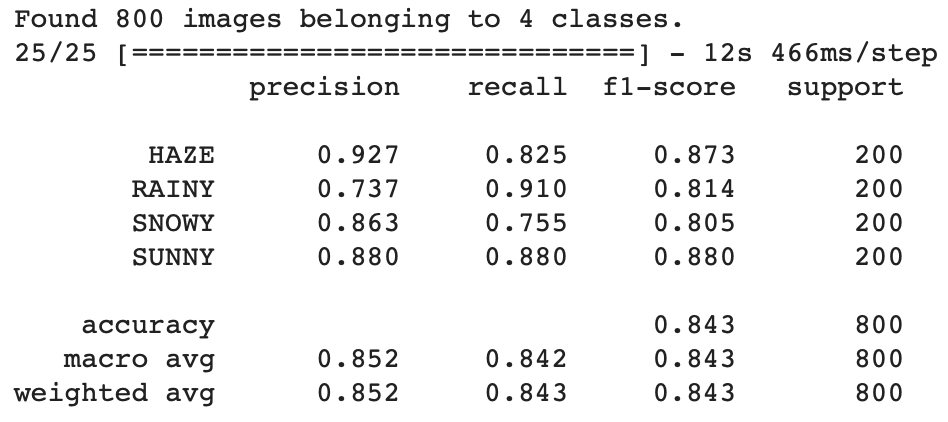
\includegraphics[width=\textwidth]{pic6}
\end{minipage}
\hspace{1em}
\begin{minipage}[c]{.5\textwidth}
   \centering
   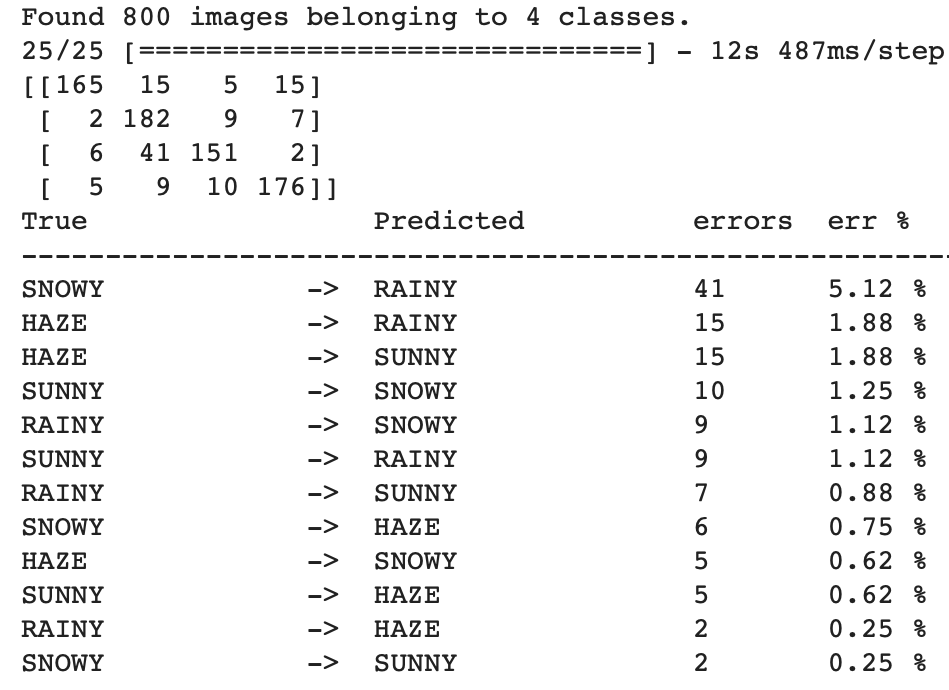
\includegraphics[width=\textwidth]{pic7}
\end{minipage}

\subsection{ValerioNet 2 - transfer model}

\bigskip
\begin{figure}[hbt!]
  \caption{{\bf ValerioNet2 Transfer $-$ Accuracy results}}
  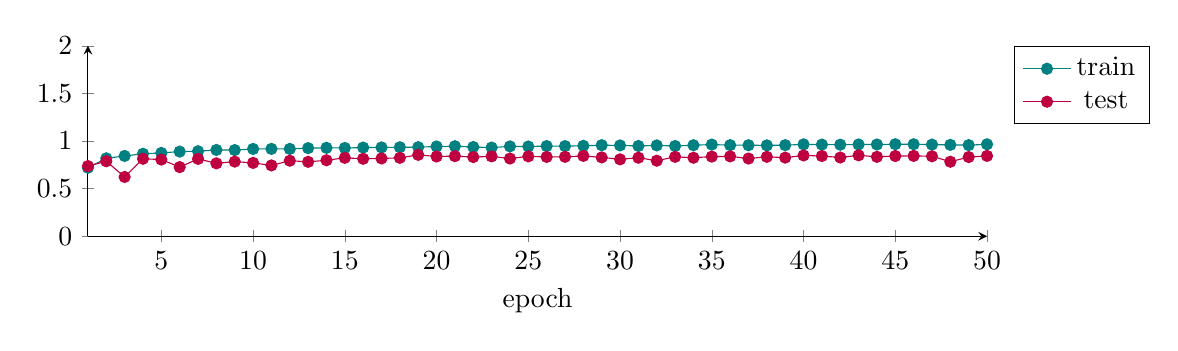
\begin{tikzpicture}
      \begin{axis}[
          width=13cm, height=4cm,
          ymin=0, ymax=2,
          xmin=1, xmax=50,
          axis x line=bottom,
          axis y line=left,
          xlabel=epoch,
          title={},
          axis on top=true, clip=false,
          legend pos=outer north east
      ]
      \addplot[mark=*, teal] coordinates {
        (1, 0.7194) (2, 0.8187) (3, 0.8434) (4, 0.8659) (5, 0.8750) (6, 0.8891) (7, 0.8931) (8, 0.9062) (9, 0.9050) (10, 0.9169) (11, 0.9175) (12, 0.9172) (13, 0.9253) (14, 0.9284) (15, 0.9269) (16, 0.9313) (17, 0.9325) (18, 0.9344) (19, 0.9356) (20, 0.9425) (21, 0.9456) (22, 0.9372) (23, 0.9309) (24, 0.9437) (25, 0.9425) (26, 0.9469) (27, 0.9469) (28, 0.9497) (29, 0.9562) (30, 0.9537) (31, 0.9481) (32, 0.9541) (33, 0.9478) (34, 0.9559) (35, 0.9628) (36, 0.9569) (37, 0.9559) (38, 0.9544) (39, 0.9566) (40, 0.9650) (41, 0.9625) (42, 0.9616) (43, 0.9637) (44, 0.9634) (45, 0.9666) (46, 0.9663) (47, 0.9625) (48, 0.9597) (49, 0.9569) (50, 0.9656)
      };
      \addplot[mark=*, purple] coordinates {
        (1, 0.7368) (2, 0.7873) (3, 0.6226) (4, 0.8137) (5, 0.8053) (6, 0.7260) (7, 0.8125) (8, 0.7656) (9, 0.7837) (10, 0.7704) (11, 0.7440) (12, 0.7933) (13, 0.7812) (14, 0.7981) (15, 0.8233) (16, 0.8137) (17, 0.8173) (18, 0.8233) (19, 0.8546) (20, 0.8377) (21, 0.8413) (22, 0.8317) (23, 0.8389) (24, 0.8161) (25, 0.8389) (26, 0.8329) (27, 0.8341) (28, 0.8438) (29, 0.8281) (30, 0.8077) (31, 0.8245) (32, 0.7933) (33, 0.8341) (34, 0.8245) (35, 0.8365) (36, 0.8389) (37, 0.8161) (38, 0.8341) (39, 0.8257) (40, 0.8486) (41, 0.8425) (42, 0.8269) (43, 0.8498) (44, 0.8341) (45, 0.8425) (46, 0.8438) (47, 0.8401) (48, 0.7825) (49, 0.8317) (50, 0.8438)
      };
      \addlegendentry{train}
      \addlegendentry{test}
      \end{axis}
  \end{tikzpicture}
\end{figure}

\bigskip
\begin{figure}[hbt!]
  \caption{{\bf ValerioNet2 Transfer $-$ Loss results}}
  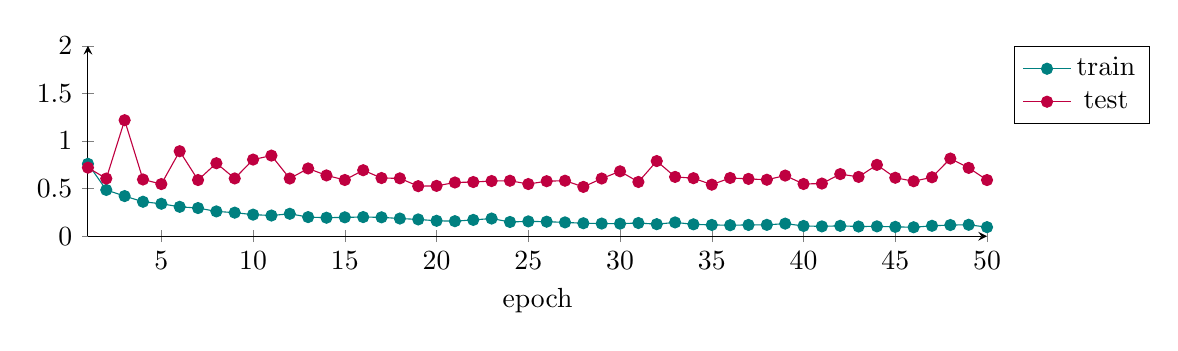
\begin{tikzpicture}
      \begin{axis}[
          width=13cm, height=4cm,
          ymin=0, ymax=2,
          xmin=1, xmax=50,
          axis x line=bottom,
          axis y line=left,
          xlabel=epoch,
          title={},
          axis on top=true, clip=false,
          legend pos=outer north east
      ]
      \addplot[mark=*, teal] coordinates {
        (1, 0.7605) (2, 0.4863) (3, 0.4218) (4, 0.3622) (5, 0.3413) (6, 0.3089) (7, 0.2961) (8, 0.2608) (9, 0.2477) (10, 0.2270) (11, 0.2177) (12, 0.2359) (13, 0.2011) (14, 0.1946) (15, 0.1986) (16, 0.2014) (17, 0.1987) (18, 0.1860) (19, 0.1767) (20, 0.1622) (21, 0.1582) (22, 0.1716) (23, 0.1858) (24, 0.1498) (25, 0.1560) (26, 0.1529) (27, 0.1454) (28, 0.1365) (29, 0.1333) (30, 0.1319) (31, 0.1389) (32, 0.1268) (33, 0.1452) (34, 0.1251) (35, 0.1188) (36, 0.1158) (37, 0.1187) (38, 0.1196) (39, 0.1325) (40, 0.1082) (41, 0.1035) (42, 0.1094) (43, 0.1022) (44, 0.1037) (45, 0.0986) (46, 0.0943) (47, 0.1095) (48, 0.1176) (49, 0.1203) (50, 0.0955)
      };
      \addplot[mark=*, purple] coordinates {
        (1, 0.7204) (2, 0.6057) (3, 1.2187) (4, 0.5961) (5, 0.5478) (6, 0.8931) (7, 0.5903) (8, 0.7668) (9, 0.6070) (10, 0.8053) (11, 0.8470) (12, 0.6062) (13, 0.7117) (14, 0.6388) (15, 0.5908) (16, 0.6934) (17, 0.6113) (18, 0.6080) (19, 0.5261) (20, 0.5290) (21, 0.5645) (22, 0.5694) (23, 0.5798) (24, 0.5830) (25, 0.5482) (26, 0.5782) (27, 0.5832) (28, 0.5183) (29, 0.6062) (30, 0.6819) (31, 0.5700) (32, 0.7896) (33, 0.6232) (34, 0.6098) (35, 0.5416) (36, 0.6122) (37, 0.6022) (38, 0.5933) (39, 0.6372) (40, 0.5488) (41, 0.5534) (42, 0.6527) (43, 0.6231) (44, 0.7497) (45, 0.6143) (46, 0.5776) (47, 0.6192) (48, 0.8160) (49, 0.7179) (50, 0.5902)
      };
      \addlegendentry{train}
      \addlegendentry{test}
      \end{axis}
  \end{tikzpicture}
\end{figure}

\newpage
Final epoch performance:
\begin{itemize}
    \item Loss: 0.0955;
    \item Accuracy: 0.9656;
\end{itemize}

Test set performance:
\begin{itemize}
    \item Loss: 0.658900;
    \item Accuracy: 0.835337;
\end{itemize}

Confusion matrix and score: \newline
\begin{minipage}[c]{.5\textwidth}
   \centering
   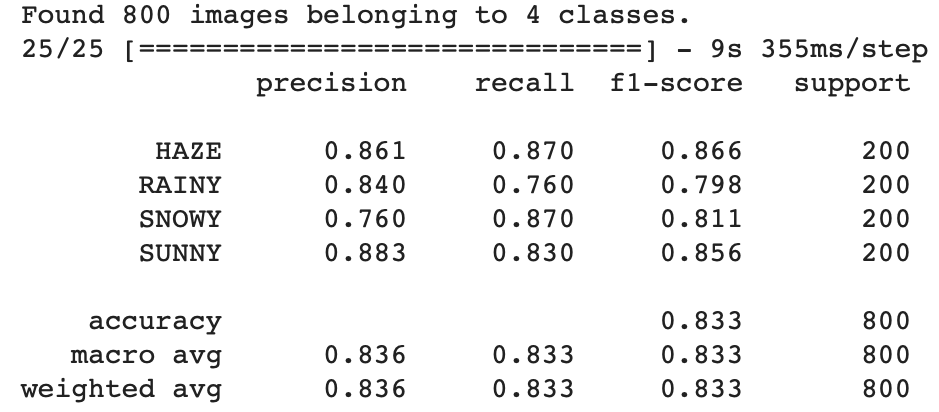
\includegraphics[width=\textwidth]{pic12}
\end{minipage}
\hspace{1em}
\begin{minipage}[c]{.5\textwidth}
   \centering
   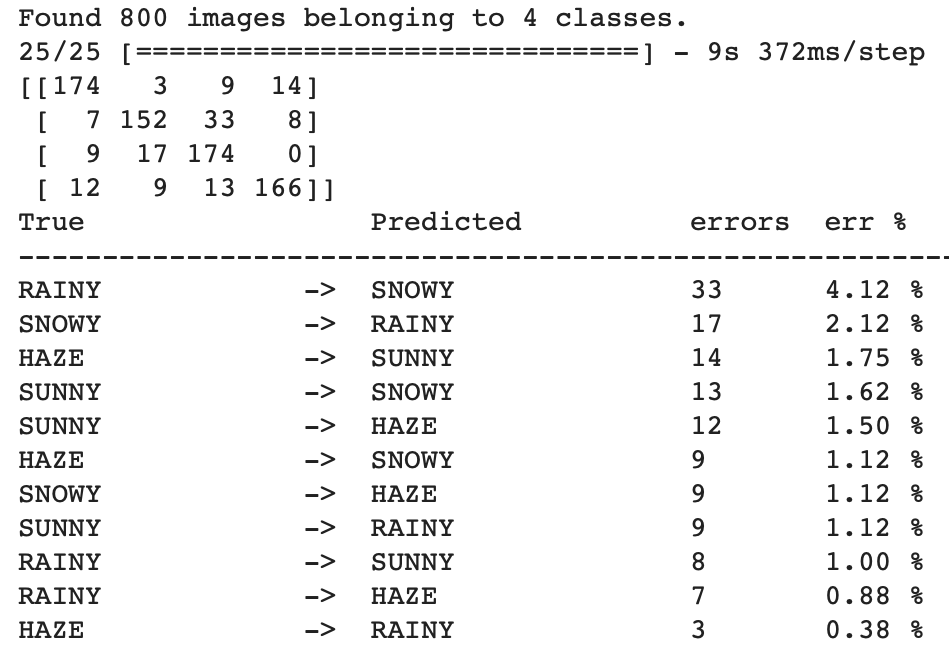
\includegraphics[width=\textwidth]{pic13}
\end{minipage}

Also in this case we have improved all the scores compared to the original model, obtaining really good results. However it turns out to be slightly worse than {\em ValerioNet1$-$Transfer Model} and this confirms the fact that ValerioNet2 was probably less stable than ValerioNet1, so we prefer the latter. For this reason, in the next sections we will only use ValerioNet1 and its transfer model to make predictions.

\newpage
\section{SMART-I Dataset}
In addition to the dataset with which we did the training we also had that of the company SMART$-$I that contains 3038 images. To test our models we therefore decided to make predictions on this dataset. Accuracy in this case is not a good measure for the evaluation since the dataset is really unbalanced: 0 {\em haze}, 521 {\em rainy}, 1421 {\em snowy}, 1096 {\em sunny}. We do the experimentation only with ValerioNet1 and relative transfer model because ValerioNet2, being unstable, does not perform very well. The following are the results:

\bigskip
{\bf ValerioNet1}: \newline
\begin{minipage}[c]{.5\textwidth}
   \centering
   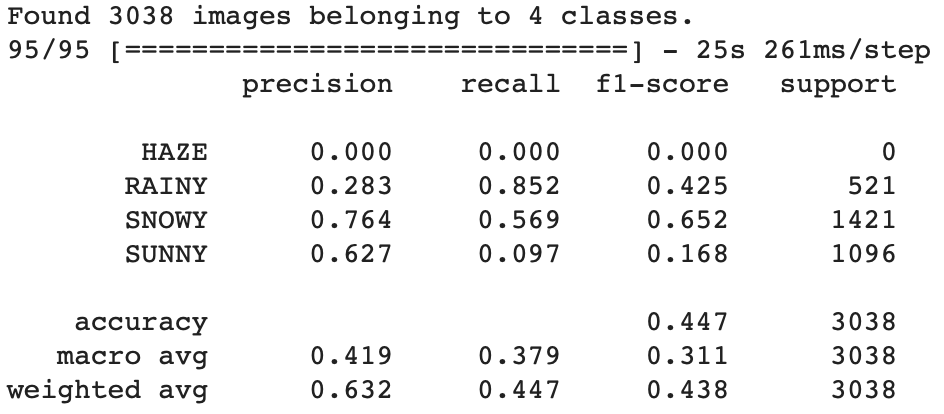
\includegraphics[width=\textwidth]{pic8}
\end{minipage}
\hspace{1em}
\begin{minipage}[c]{.5\textwidth}
   \centering
   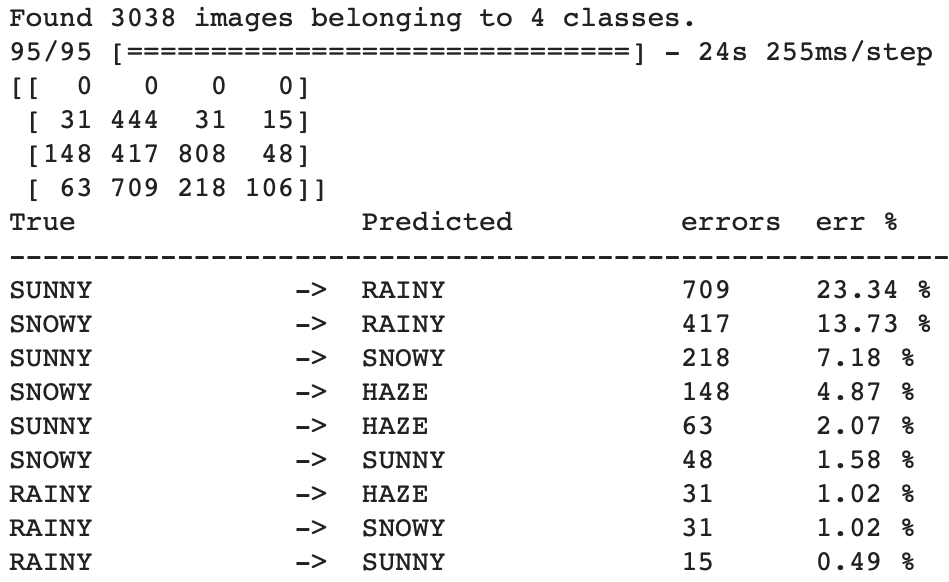
\includegraphics[width=\textwidth]{pic9}
\end{minipage}

Test set performance:
\begin{itemize}
    \item Loss: 4.196499;
    \item Accuracy: 0.447005;
\end{itemize}

\bigskip
{\bf ValerioNet1$-$Transfer Model} \newline
\begin{minipage}[c]{.5\textwidth}
   \centering
   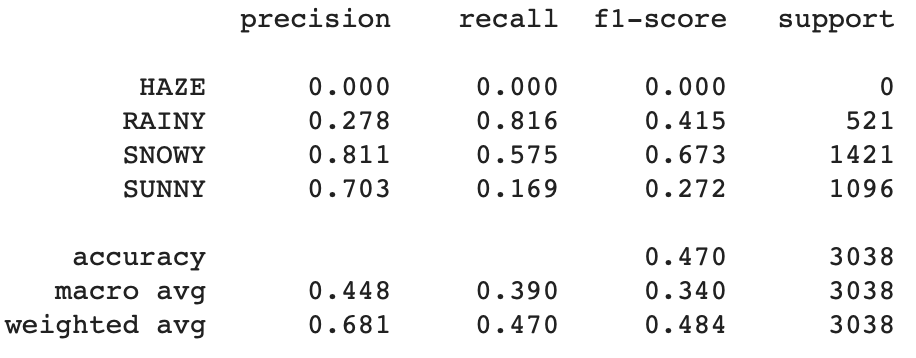
\includegraphics[width=\textwidth]{pic10}
\end{minipage}
\hspace{1em}
\begin{minipage}[c]{.5\textwidth}
   \centering
   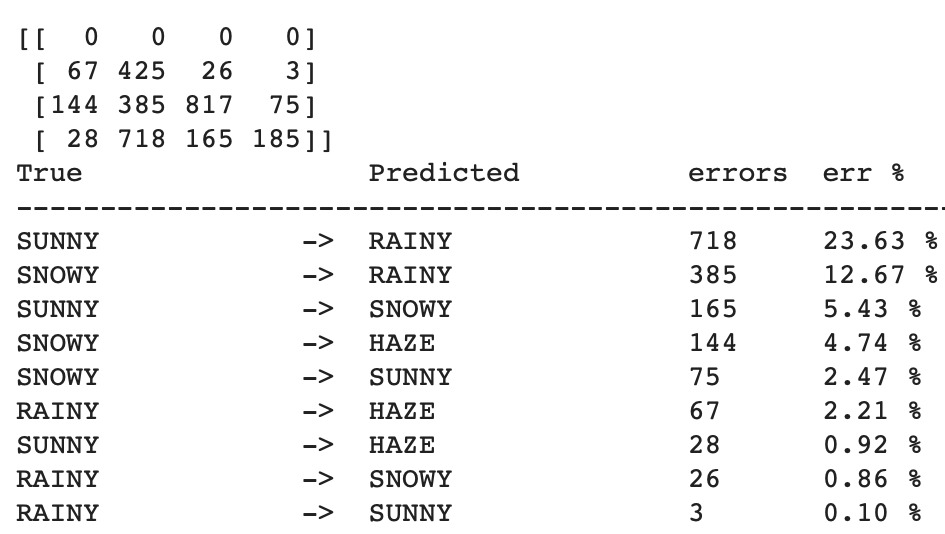
\includegraphics[width=\textwidth]{pic11}
\end{minipage}

Test set performance:
\begin{itemize}
    \item Loss: 3.305563;
    \item Accuracy: 0.469717;
\end{itemize}

In both cases we do not have good performances but we directly analyze those of {\em ValerioNet1$-$Transfer Model} which are slightly better.
Being the dataset unbalanced, we take the weighted average of the various scores, and we see that the images classified as correct only 68\% were really correct, instead of all the corrected images only 47\% were classified as correct. The misclassification of sunny as rainy and snowy as rainy is the most common error. So with this dataset our models seem to classify the images as more rainy than they should be.

However, even if the results are not very good, this test helped us to confirm ValerioNet1-Transfer Model as the final model.

\newpage
\section{Conclusion}

We report in a table the results:

\bigskip
\begin{tabular}{ | l | l | l | l | l | }
    \hline
    \textbf{Model} & \textbf{Input Shape} & \textbf{Accuracy} & \textbf{Loss} \\ \hline
    \textbf{LeNet}          & 200x200 & 0.679087 & 0.912283  \\ \hline
    \textbf{AlexNet}        & 118x224 & 0.634615 & 1.742811  \\ \hline
    \textbf{ValerioNet1}    & 200x200 & 0.769231 & 0.870954  \\ \hline
    \textbf{ValerioNet2}    & 200x200 & 0.801683 & 0.691415  \\ \hline
    \textbf{ValerioNet1 TL} & 200x200 & 0.842548 & 0.655136  \\ \hline
    \textbf{ValerioNet2 TL} & 200x200 & 0.835337 & 0.658900  \\ \hline
\end{tabular}
\bigskip

As we can see ValerioNet1$-$TL is the best and for this reason we have chosen it to make the predictions in the blind set.
\vfill

\begin{thebibliography}{99}

\bibitem{kerasdoc}
{\em Keras Documentation}.\newline
  \verb|https://keras.io|

\bibitem{lenet}
{\em LeNet-5 – A Classic CNN Architecture}.\newline
  \verb|https://engmrk.com/lenet-5-a-classic-cnn-architecture/|

\bibitem{alexnet}
{\em Understanding AlexNet}.\newline
  \verb|https://www.learnopencv.com/understanding-alexnet/|

\bibitem{transfer learning}
{\em Transfer Learning - Wikipedia}.\newline
  \verb|https://en.wikipedia.org/wiki/Transfer_learning|

\end{thebibliography}
\end{document}
